\documentclass{article}
\usepackage{amsmath,amsthm}
\usepackage{amssymb}
\usepackage{listings}
\usepackage{flexisym}
\usepackage{graphicx}
%\usepackage{titling}
\makeatletter
\def\tagform@#1{\maketag@@@{[\ignorespaces#1\unskip\@@italiccorr]}}
\makeatother
\title{The Essence of Pushdown Control Flow Analysis \\ and Efficient Application for JavaScript Analysis}
\author{Fei Peng}
\begin{document}
\maketitle
%\tableofcontents
\begin{abstract}
In traditional control flow analysis area, call/return mismatch is always a problem that dramatically reduces precision of analysis. Although, original \textit{k}-CFA uses bounded call strings to acquire limited call/return exact match, this technique causes serious performance cost due to it coupling call/return match strategies with context-sensitivity of values.
Meanwhile, abstracting abstract machine (AAM) a configurable framework for constructing abstract interpreters introduces store-allocated continuation that makes soundness of abstract interpreters easily acquired. Recently, there are three different approaches (PDCFA, AAC, and P4F) published, which provide perfect call/return match for AAM via modeling call stacks as pushdown systems. However, PDCFA needs extra annotated edges to represent stack actions that leads implementing become difficult. AAC requires expensive overhead, and P4F cannot work with monovariance (0-CFA). Consequently, we developed a new method to address the call/return mismatch problem that is extremely easy to implement for ANF style program in abstracting abstract machine. Simultaneously, this method reveals the essence of pushdown control flow analysis, and we exploit the essence to develop a static analyzer for JavaScript with direct abstract syntax tree.

\end{abstract}
\section{Introduction}
\label{Introduction}
Dynamic programming languages (e.g. JavaScript, Python, and Ruby, etc.) play a significant role in a lot of computing areas, such as system management, web development, and scientific computing. Especially, in the past decade, JavaScript becomes a ubiquitous computing environment. However, their certain features (e.g.\ duck-typing, first-class function, highly dynamic object model) make bug detection difficult. Control flow  analysis becomes a good approach to detect deeply semantic defeats before actual running programs, but original control flow analysis (\textit{k}-CFA) is too imprecise to apply in realized programs. For example, call/return mismatch is always a problem in \textit{k}-CFA that dramatically reduces precision of analysis.

\lstset{language=Lisp, mathescape}
\begin{lstlisting}

  (let* ((id (lambda (x) x))
         (a (id 1)$^1$)
         (b (id #t)$^2$))
      a)

\end{lstlisting}


Let's consider about the trivial example, in traditional 0-CFA the id function is called twice and \#t finally flows into variable a because there is a spurious flow from call site (id \#t) return to (a (id 1)). In \textit{k}-CFA (k $\geq$ 1), the values of local variable x are distinguished by different call site environments. To illustrate, $(x, 2) \longrightarrow \#t$ means that the value of x is \#t in call site 2, and original \textit{k}-CFA also can use the values' environment to filter inter-procedure control flows, which value of x from call site 2 only can be returned to (b (id \#t)). In this case (non-recursive program), call string with finite length is enough for providing precise call/return flow (value and control flow both). However, any recursive function call will break the rule and propagate spurious information to the whole program. Meanwhile, the performance is unacceptable even when k is 1.

The core idea of pushdown control flow analysis is to mimic call/return flow as a unbounded call stack for ordinary calls, and summarizes the call stack for recursive calls because unbounded call stack is uncomputable in static analysis. CFA2 implements the summarization with a tabulate algorithm, and PDCFA annotates state transition edges with stack actions (push, pop, and no action).Both of CFA2 and PDCFA introduce extra semantics for target languages that makes the abstract interpreters hard to implement.
Fortunately, XXX invented abstracting abstract machine (AAM) as a configurable framework for constructing abstract interpreters in the CESK abstract machine style. AAM not only allocate values in the store (like original \textit{k}-CFA does), but also represents control flow as store-allocated continuations. In AAM, each CESK state does not directly carry continuation, but a continuation address refers to a set of continuations in the store. Merging serval continuations in one continuation address achieves approximation of control flows. Meanwhile, AAM brings two benefits to control flow analysis. On the one hand, it makes soundness of abstract interpreters easily acquired because values and continuations are both in the store and the store size is fixed. On the other hand, store-allocated traditional separates original context-sensitivity (polyvariant values) strategies from call/return match techniques.
AAC and P4F both based on AAM convert call/return match problem to continuation address allocation strategy. AAC requires expensive overhead, $O(n^9)$, which puts too much information in the continuation addresses. Then P4F tries to reduce the complexity of AAC, but it is not useful for monovariant analysis.

In this paper, we introduce a new method to address the call/return mismatch problem that is as simple as P4F and AAC, and it can provide perfect call/return match for monovariant and polyvariant control flow analysis. The new method puts a \emph{execution history environment} into continuation address with callee's function boy, so we name it \textit{h}-CFA . The execution history environments can be regarded as call strings with automatically determined length. For non-recursive calls, execution history always provides enough precise context information, no matter how deep the call sequences. On the other hand, execution history can automatically stop growth for recursive calls, and the work list algorithm will be responsible for finding the fixed-point of recursive computation.



\begin{figure}[t]
\small
\begin{center}
\begin{tabular}{ccc}
%\raisebox{1ex-\height}{
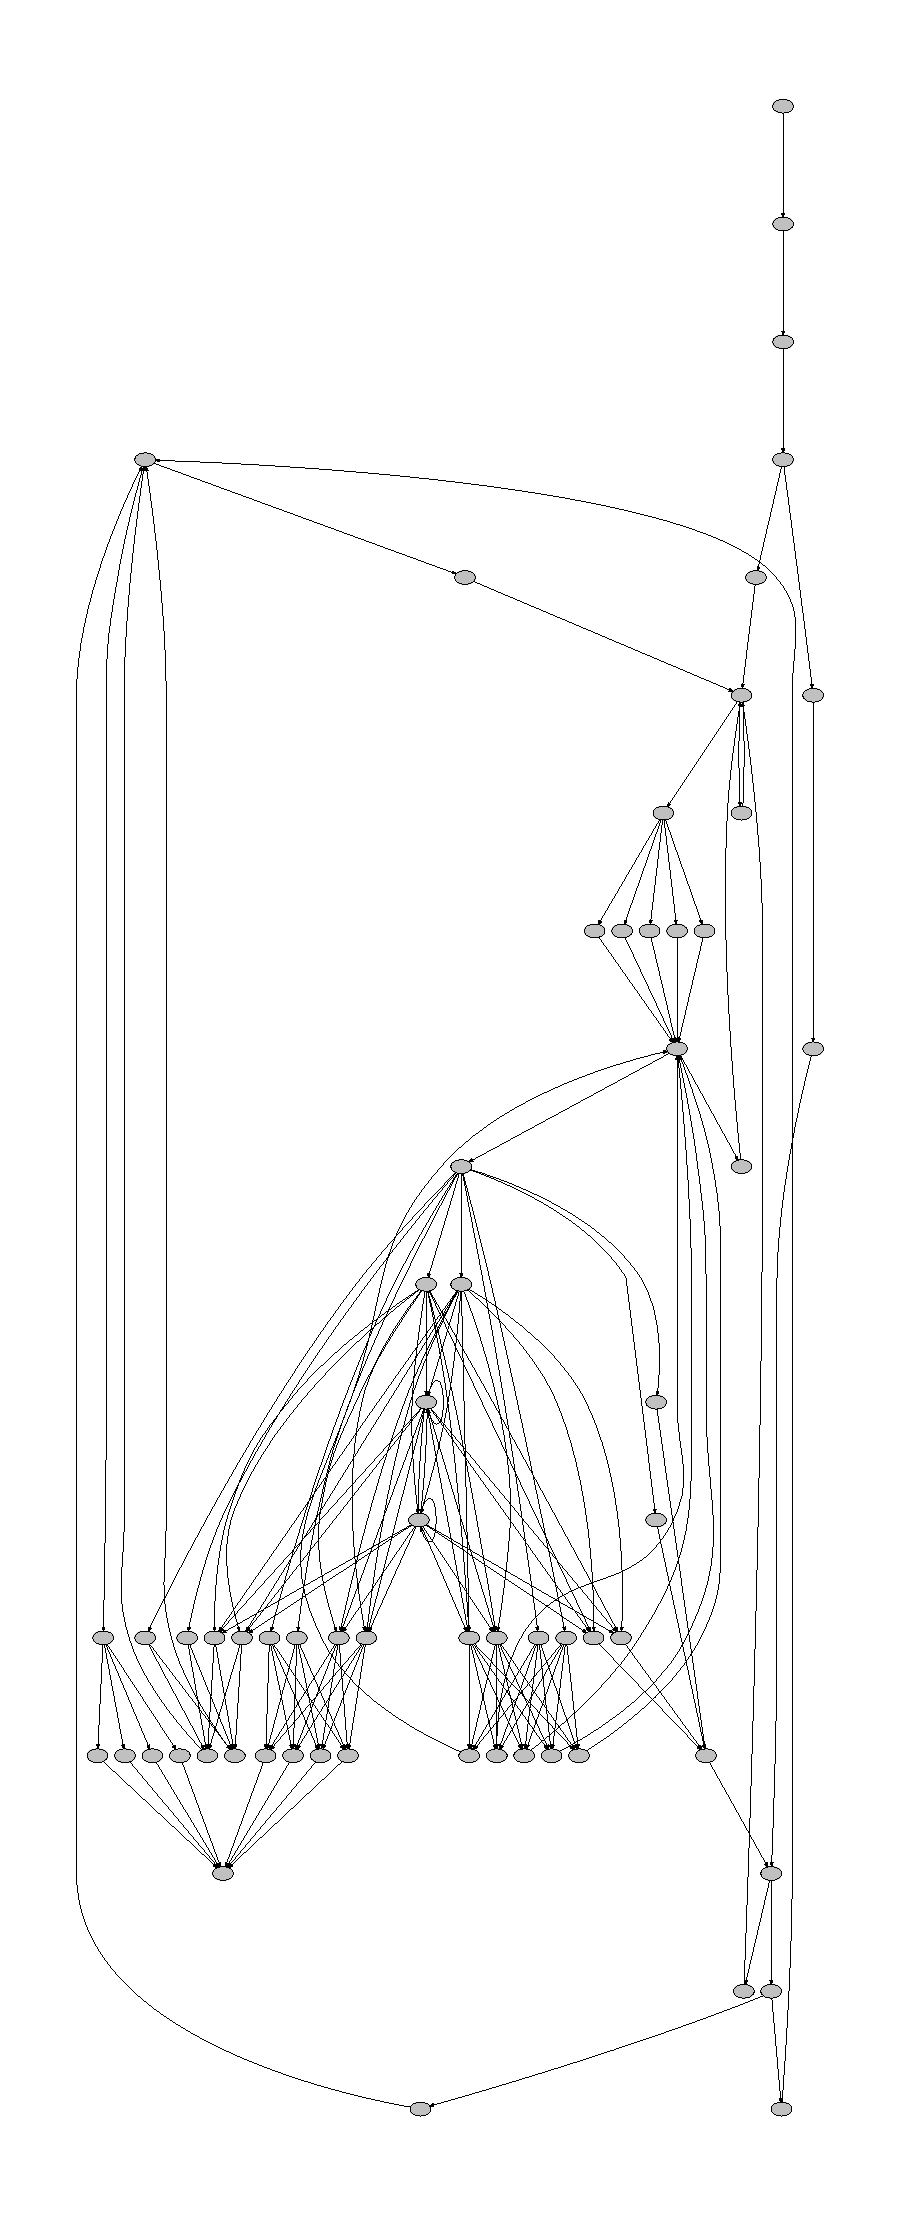
\includegraphics[height=3.5in]{1p4f.pdf}
%}
&
%\raisebox{1ex-\height}{
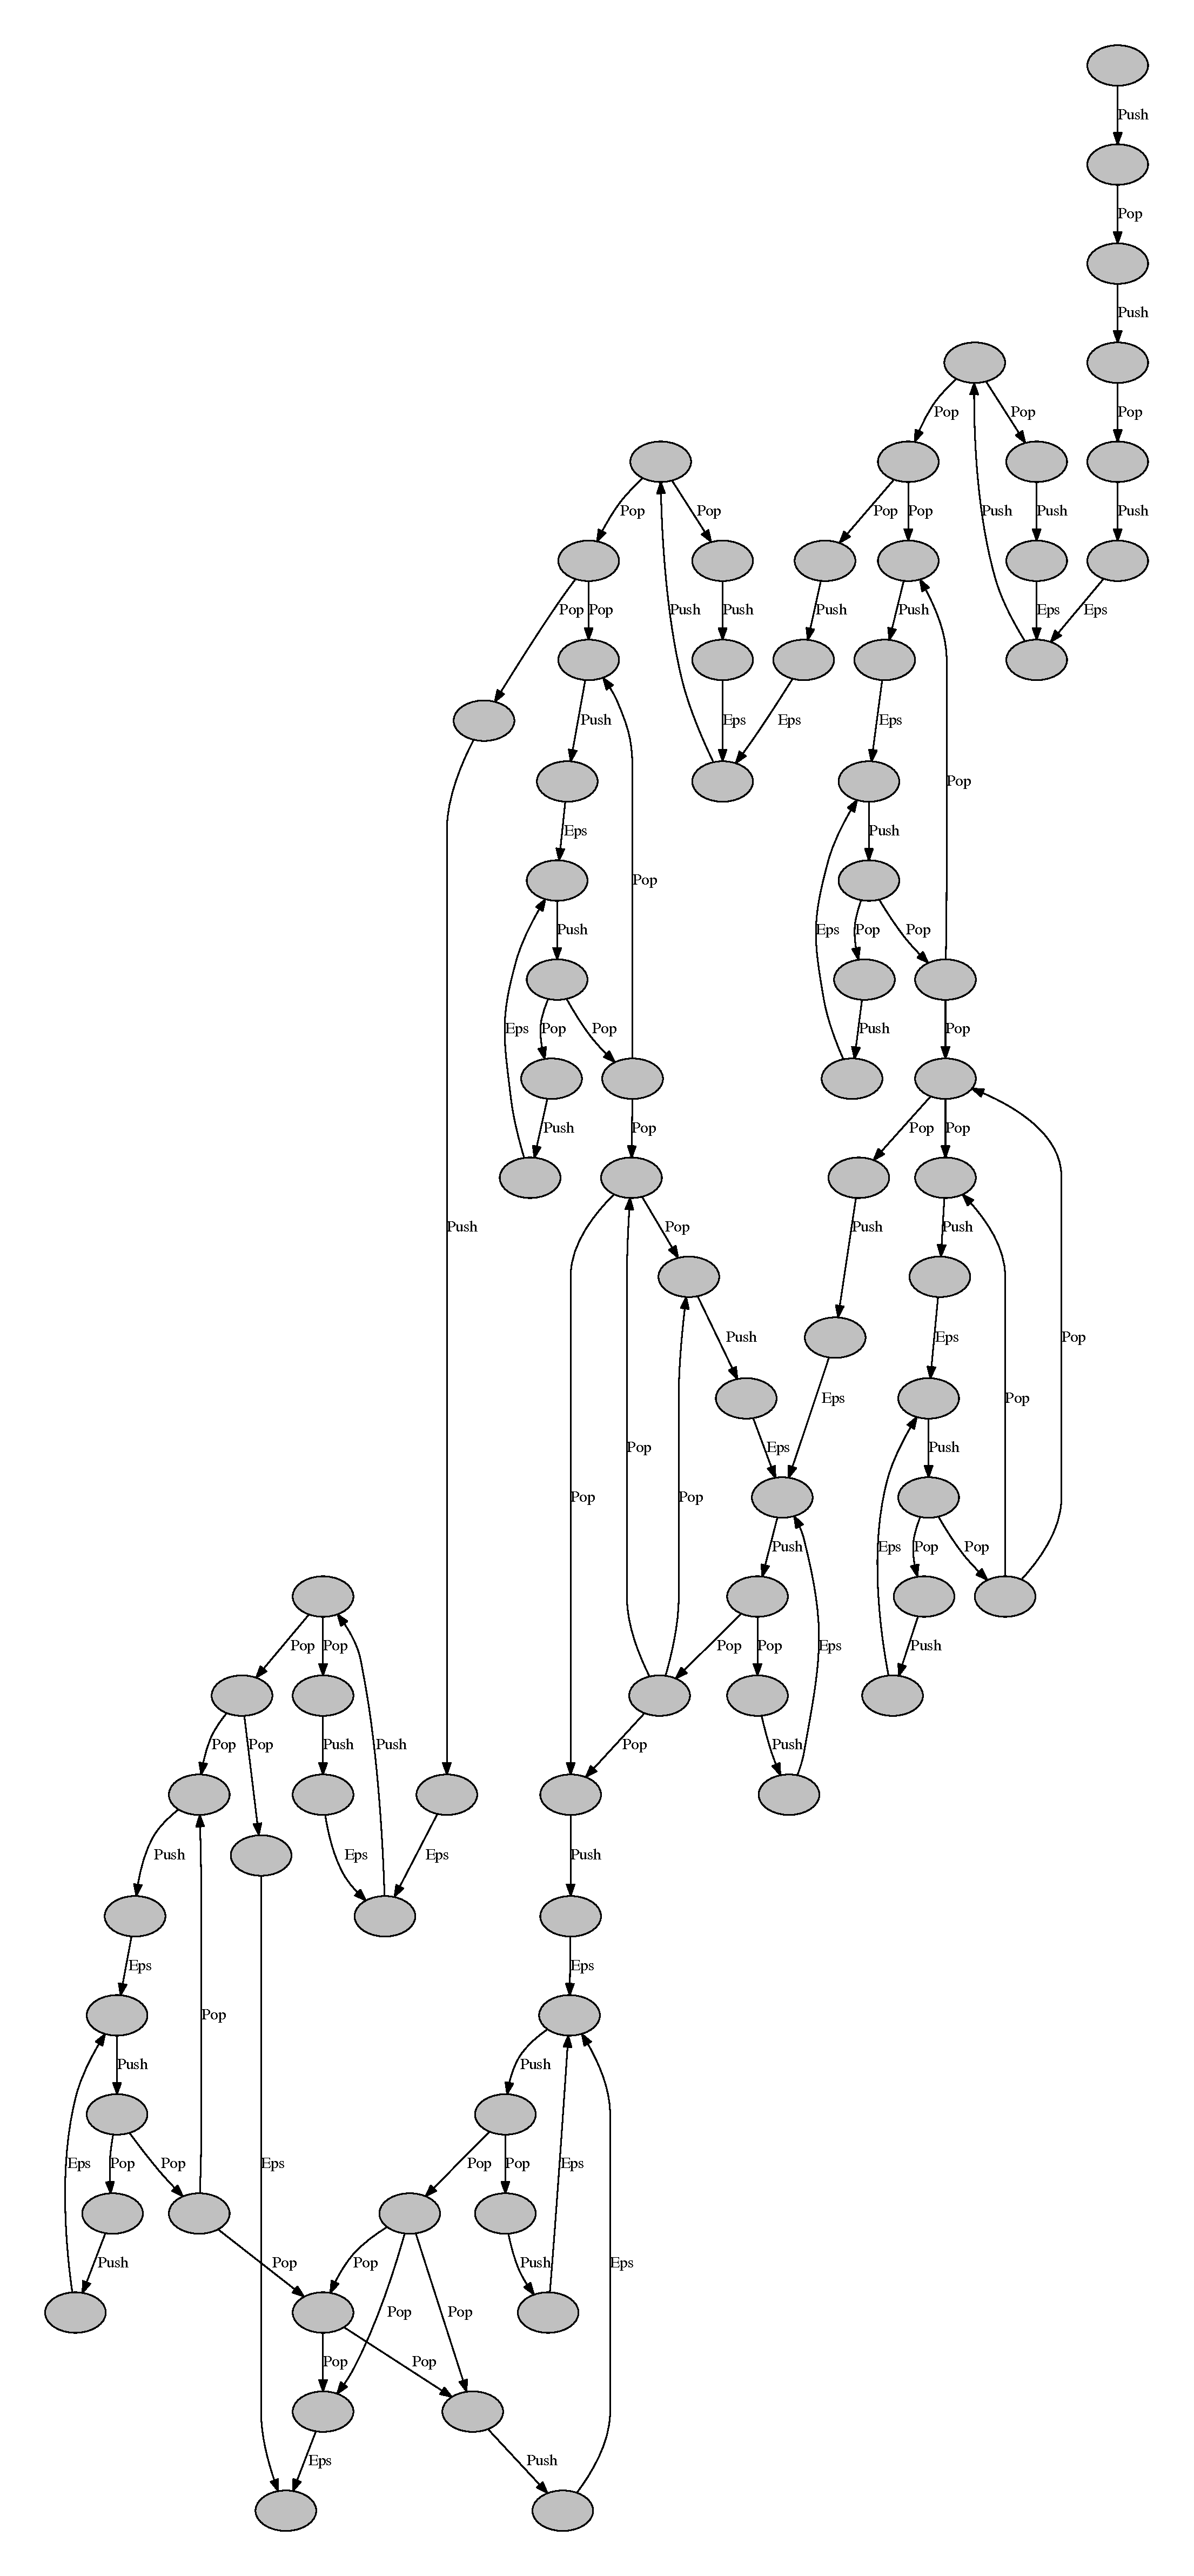
\includegraphics[height=3.5in]{pdcfaWOgc.pdf}
%}
\\
(a) P4F with 1-call-sensitive
&
(b) PDCFA
\\
%\raisebox{1ex-\height}{
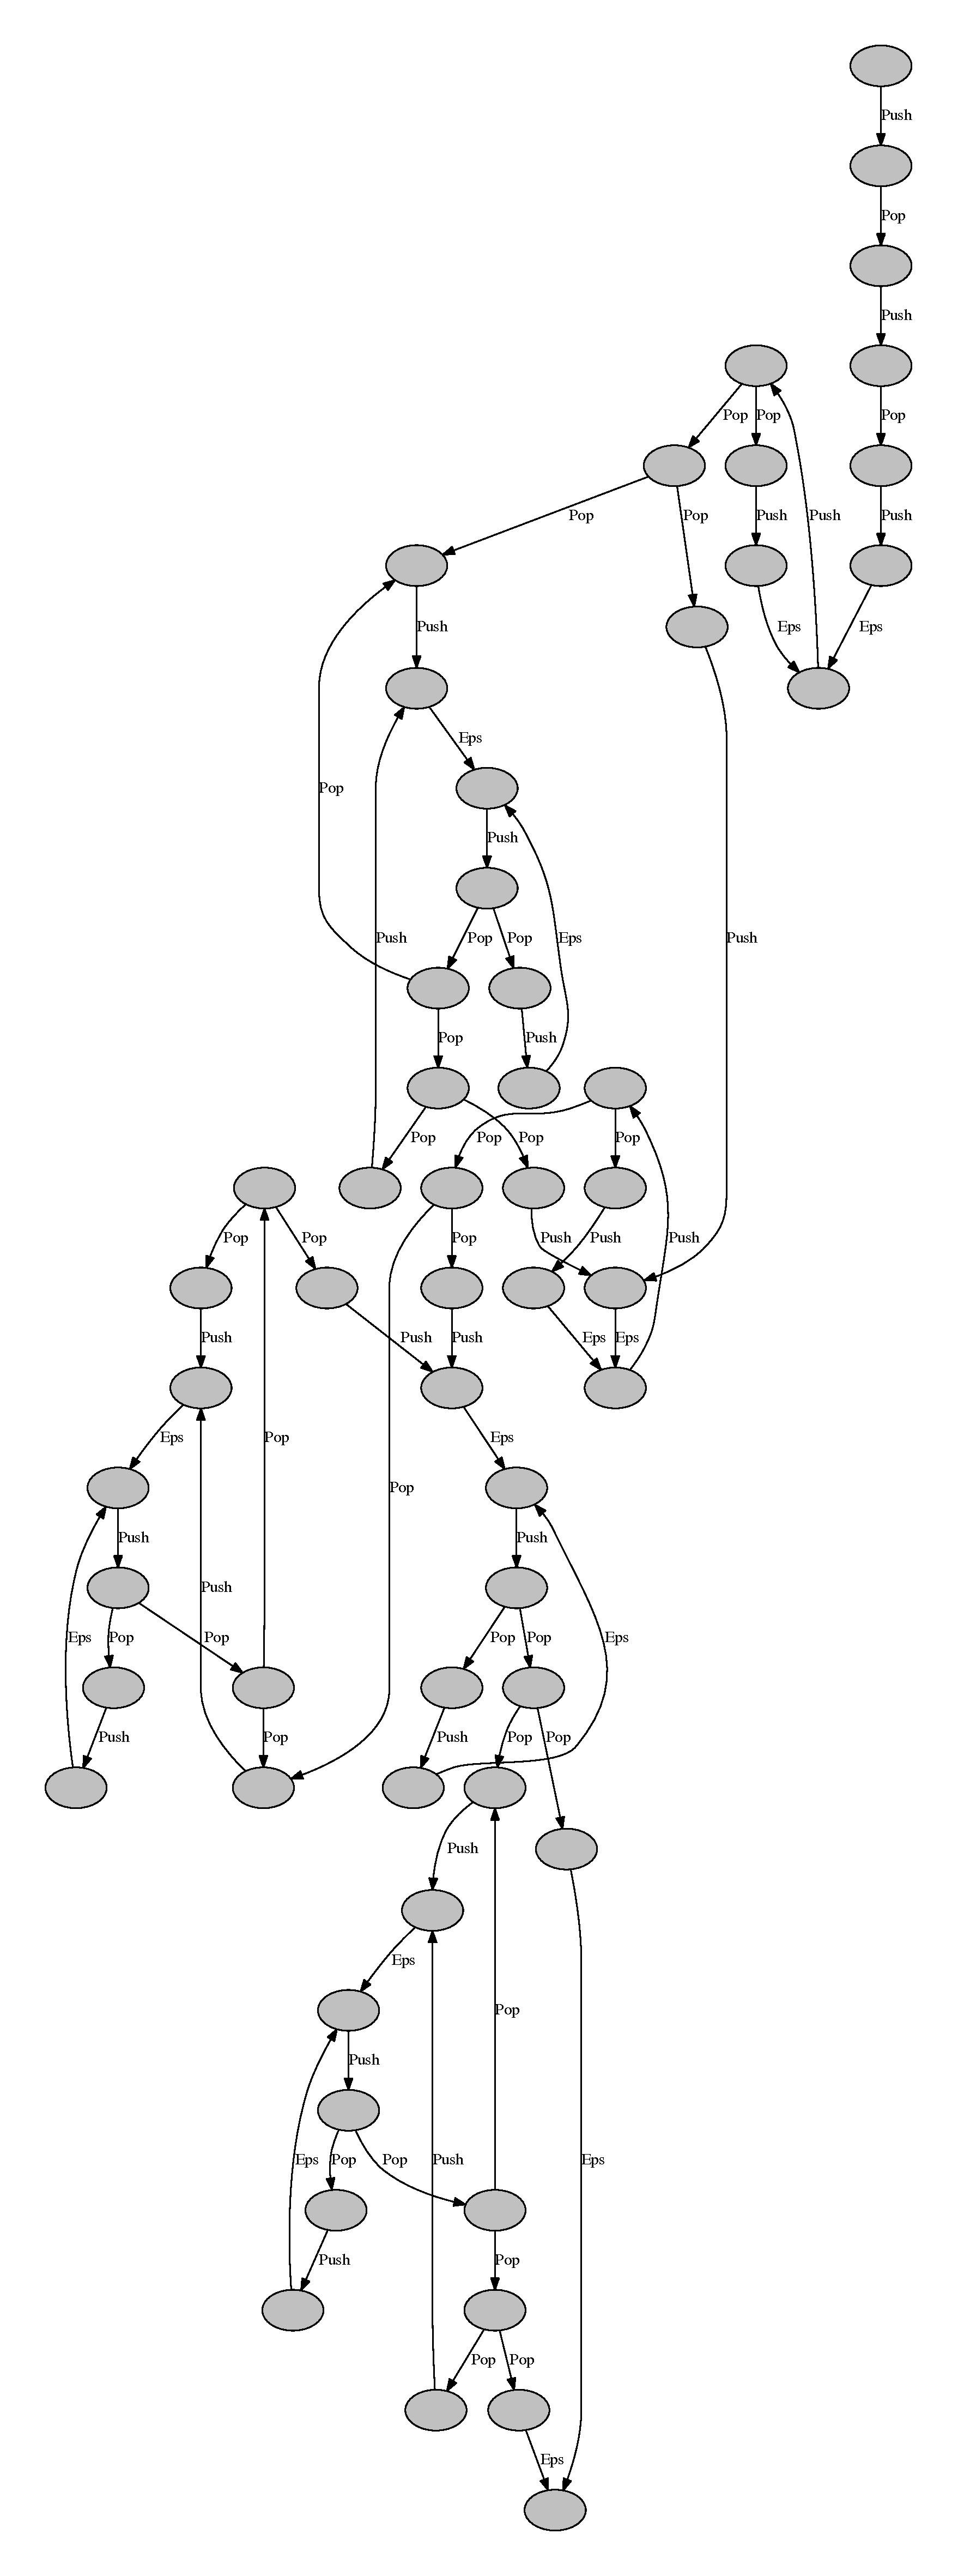
\includegraphics[height=3in]{pdcfa.pdf}
%}
&
%\raisebox{1ex-\height}{
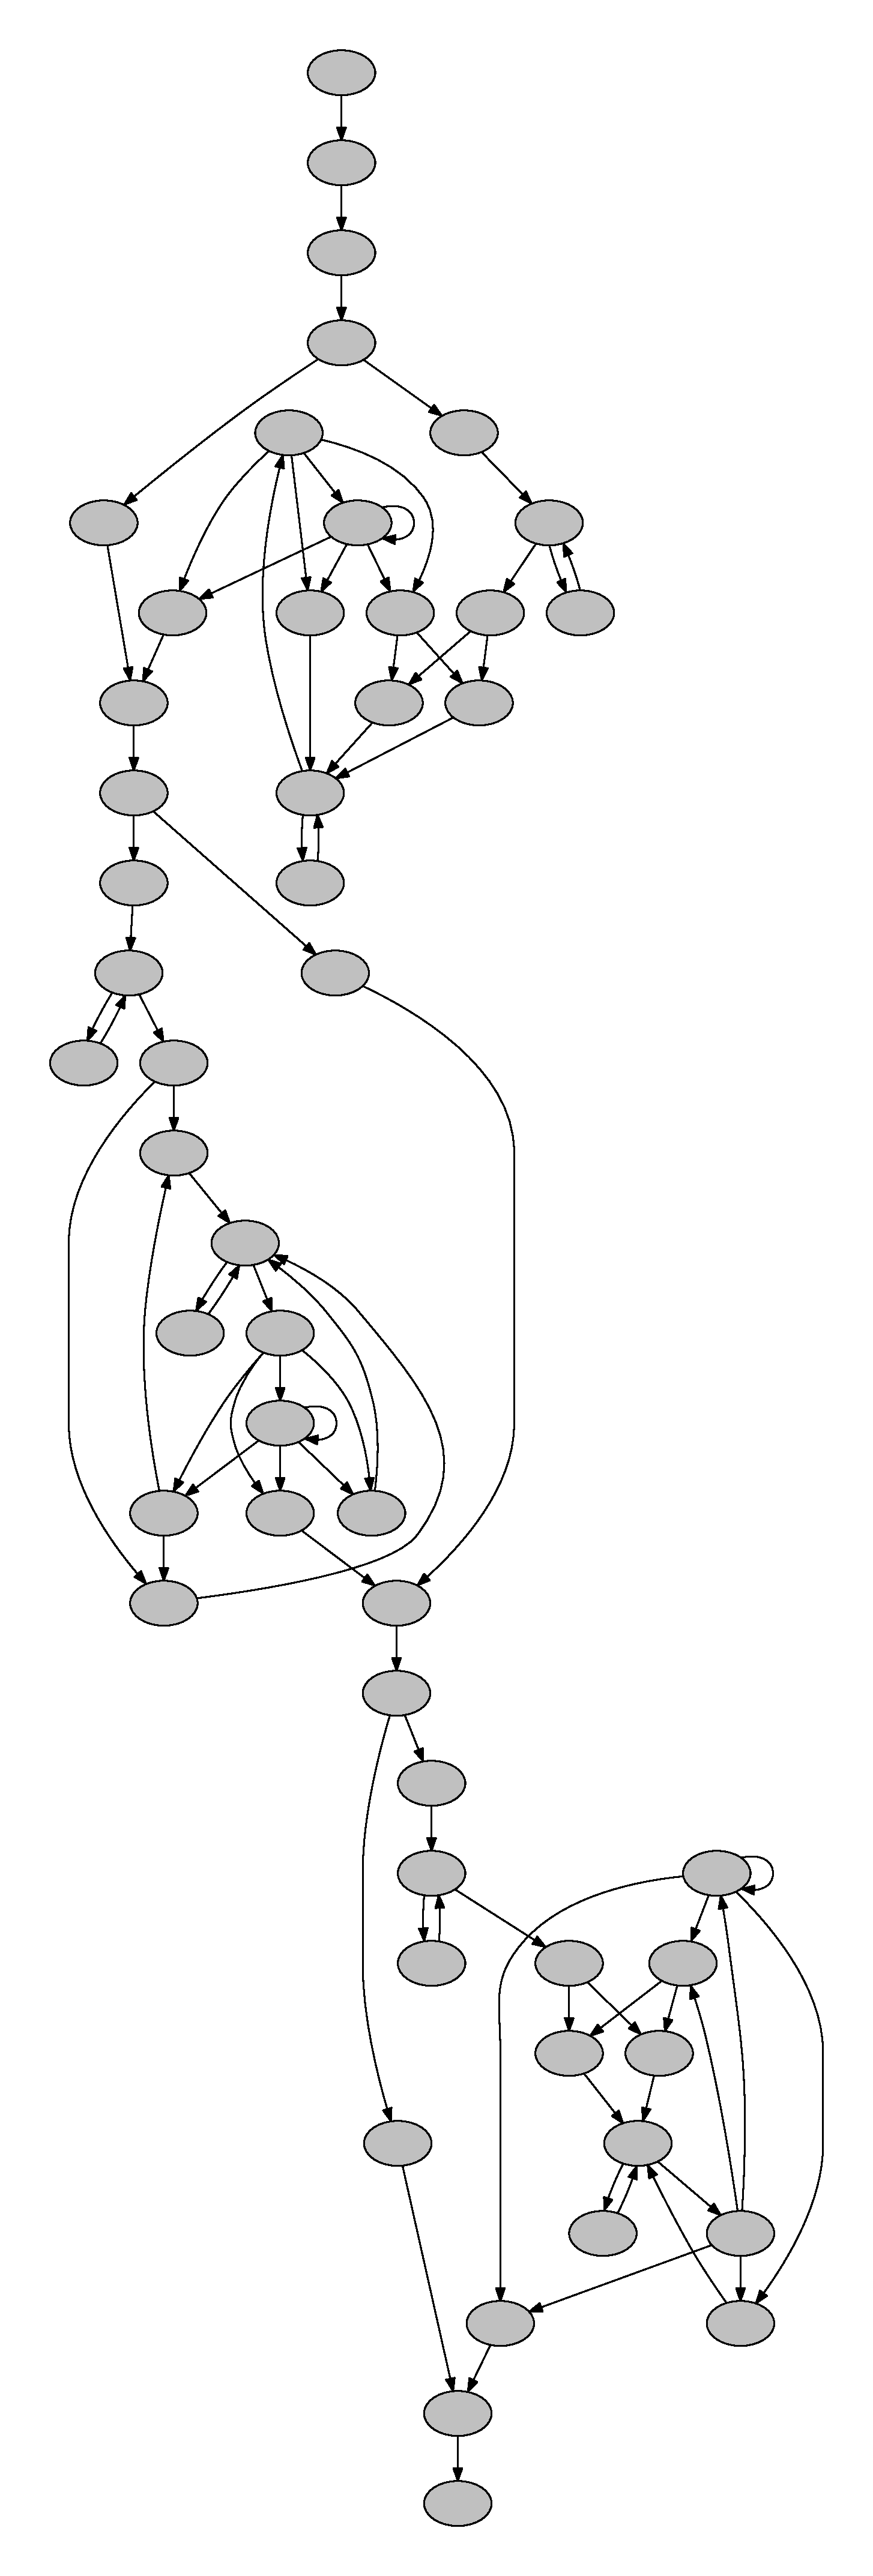
\includegraphics[height=3in]{ncfa.pdf}
%}
\\
(c) PDCFA with Abstract Garbage Collection
&
(d) \textit{h}-CFA
\end{tabular}
\end{center}
\caption{
(a) shows
}
\label{fig:state-graphs}
\end{figure}


\section{Pushdown Control Flow Analysis in Abstracting Abstract Machines}
\label{sec:Pushdown Control Flow Analysis in Abstracting Abstract Machines}
\subsection{Abstracting Abstract Machine}
\label{subs:Abstracting Abstract Machine}
Before section 4, we will describe algorithms on ANF style lambda calculus.
\[\begin{aligned}
e \in Exp ::= (let ((x (f e))) e) \\
            | e
\end{aligned}
\]
\[
\tag{atomic expressions}
f, e \in AExp ::= x\ |\ lambda
\]
\[
\tag{lambda abstractions}
lambda \in Lambda ::= (\lambda (x) e)
\]
\[
\tag{variables}
x,y \in Var \ is\ a\ set\ of\ identifiers
\]

This section reviews AAM .
\subsection{A defeat of AAM}
\label{sub:A defeat of AAM}
Although, abstracting abstract machines import store-allocated values and store-allocated continuations that make call/return match orthogonal from context-sensitivity, original ``kalloc'' functions (continuation address allocating strategy) cannot depend upon context information to implement limited call/return match (like \textit{k}-CFA does). P4F attempts to narrow the gap between original \textit{k}-CFA and AAM, so it defines the very simple ``kalloc'' function:

\[
\widetilde{kalloc_{P4F}} ((e, \widetilde{\rho}, \widetilde{\sigma}, \widetilde{\sigma_k}, \widetilde{a_k}), e\textprime, \widetilde{\rho}\textprime, \widetilde{\sigma}\textprime) = (e\textprime, \widetilde{\rho}\textprime)
\]

P4F adepts
\section{The Essence of Pushdown Control Flow Analysis}
\label{sec:The Essence of Pushdown Control Flow Analysis}
\subsection{Program Execution History}
\label{sub:Program Execution History}
Definitions:

\[
\tag{states}
\widetilde{\varsigma}\in\widetilde{\Sigma} \triangleq Exp \times \widetilde{Env} \times \widetilde{Store}
\times \widetilde{KStore} \times \widetilde{KAddr} \times \widetilde{History}
\]
\[
\tag{environments}
\widetilde{\rho} \in \widetilde{Env} \triangleq Var \rightharpoonup \widetilde{Addr}
\]
\[
\tag{srores}
\widetilde{\sigma} \in \widetilde{Store} \triangleq \widetilde{Addr} \to \widetilde{Value}
\]
\[
\tag{abstract values}
\widetilde{v} \in \widetilde{Value} \triangleq \mathcal{P}(\widetilde{Closure})
\]
\[
\tag{closures}
\widetilde{clo} \in \widetilde{Closure} \triangleq Lambda \times \widetilde{Env}
\]
\[
\tag{continuation stores}
\widetilde{\sigma_k} \in \widetilde{KStore} \triangleq  \widetilde{KAddr} \to  \widetilde{Kont}
\]
\[
\tag{abstract continuations}
\widetilde{k} \in  \widetilde{Kont} \triangleq  \mathcal{P}(\widetilde{Frame})
\]
\[
\tag{stack frames}
\widetilde{\phi} \in  \widetilde{Frame} \triangleq Var \times Exp \times  \widetilde{Env} \times \widetilde{History} \times  \widetilde{KAddr}
\]
\[
\tag{histories}
\widetilde{h} \in \widetilde{History} \triangleq Var \rightharpoonup \widetilde{Addr}
\]
\[
\tag{value addresses}
\widetilde{a} \in \widetilde{Addr} \ is\ a\ finite\ set
\]
\[
\tag{continuation addresses}
\widetilde{a_k} \in \widetilde{KAddr} \ is\ a\ finite\ set
\]

Abstract Semantics:

kalloc:
\[
\widetilde{kalloc_h} ((e, \widetilde{\rho}, \widetilde{\sigma}, \widetilde{\sigma_k}, \widetilde{a_k}, \widetilde{h}), e\textprime, \widetilde{\rho}\textprime, \widetilde{\sigma}\textprime) = (e\textprime, \widetilde{h})
\]

calls:
\[
\overbrace{
\big((let\ ([y\ (f\ ae)]\ e)), \widetilde{\rho}, \widetilde{\sigma}, \widetilde{\sigma_k}, \widetilde{a_k}, \widetilde{h} \big)
}^{\widetilde{\varsigma}}
\leadsto \big(e\textprime,\widetilde{\rho}\textprime, \widetilde{\sigma}\textprime, \widetilde{\sigma_k}\textprime, \widetilde{a_k}\textprime, \widetilde{h}\textprime \big), where
\]
\[
\big((lambda\ (x)\ e\textprime), \widetilde{\rho}_{\lambda}  \big) \in \widetilde{eval}(f, \widetilde{\rho}, \widetilde{\sigma})
\]
\[
\widetilde{\rho}\textprime = \widetilde{\rho}_{\lambda}[x \to \widetilde{a}]
\]
\[
\widetilde{\sigma}\textprime = \widetilde{\sigma} \sqcup [\widetilde{a} \to \widetilde{eval}(ae, \widetilde{\rho}, \widetilde{\sigma})]
\]
\[
\widetilde{a} = \widetilde{alloc}(x, \widetilde{\varsigma})
\]
\[
\widetilde{\sigma_k}\textprime = \widetilde{\sigma_k} \sqcup [\widetilde{a_k}\textprime \to {(y, e, \widetilde{\rho}, \widetilde{h}, \widetilde{a_k})}]
\]
\[
\widetilde{a_k}\textprime = \widetilde{kalloc}(\widetilde{\varsigma}, e\textprime, \widetilde{\rho}\textprime, \widetilde{\sigma}\textprime)
\]
\[
\widetilde{h}\textprime = \widetilde{h} \cup \widetilde{\rho}  \cup \widetilde{\rho}\textprime
\]

returns:
\[
\overbrace{
(ae, \widetilde{\rho}, \widetilde{\sigma}, \widetilde{\sigma_k}, \widetilde{a_k}, \widetilde{h})
}^{\widetilde{\varsigma}}
\leadsto (e, \widetilde{\rho}\textprime, \widetilde{\sigma}\textprime, \widetilde{\sigma_k}, \widetilde{a_k}\textprime, \widetilde{h}\textprime)
\]
\[
(x, e, \widetilde{\rho_k}, \widetilde{h_k}, \widetilde{a_k}\textprime) \in \widetilde{\sigma_k}(\widetilde{a_k})
\]
\[
\widetilde{\rho}\textprime = \widetilde{\rho_k}[x \to \widetilde{a}]
\]
\[
\widetilde{\sigma}\textprime = \widetilde{\sigma} \sqcup [\widetilde{a} \to \widetilde{eval}(ae, \widetilde{\rho}, \widetilde{\sigma})]
\]
\[
\widetilde{a} = \widetilde{alloc}(x, \widetilde{\varsigma})
\]
\[
\widetilde{h}\textprime = \widetilde{h_k} \cup \widetilde{\rho}\textprime
\]

\subsection{Polyvariant Continuation}
\label{sub:Polyvariant Continuation}
In this section, we use illustrations to show the principles of \textit{h}-CFA.
\section{Static Analysis of JavaScript}
\label{sec:Static Analysis of JavaScript}
\subsection{Abstract Garbage Collection as Stack Filtering}
\label{sub:Abstract Garbage Collection as Stack Filtering}
In practice, call/return perfect match working with monovariant analysis is useless.
\subsection{Abstract Garbage Collection as Popping Call Stack Frames}
\label{sub:Abstract Garbage Collection as Popping Call Stack Frames}
In this section, we show how to give up execution history and apply our theory for direct-style AST.
\end{document}
